Up to this chapter, our focus has been on the fullfillment of a constraint given in terms of production rate and production time. In this part of the course, we will change our main objective by adding a constraint on the number of items to be produced. Still we will have a minimum rate to be performed, stil we will have a production time limit not to be crossed, but the objective now becomes to produce exactely $N$ final products and to plan the production accordingly. 

\section{Given that $b_i = b_fn_{if}$}

\subsection{Push systems}

We know, from the previous chapters, that the production time can be computed as \[ T_{prod}(b_f) = \max_{\mathcal P_k}\left( \sum_{i\in\mathcal P_k}(T_{si} + b_fT_{oi}n_{if}) \right) \] but it is worthy to notice that the time to seperately produce two batches of size $b_f$ does not equal the double time we would need to produce one batch of size $b_f$. More formally, we are saying that $T_{prod}(2.b_f)|_{b_f}\ne 2T_{prod}(b_f)$ in the sense that figure (\ref{produced_i:2bf}) represents. In fact, we do not need for a whole "production cycle" to be finished to begin with another one. Indeed, we can begin a new cycle as soon as the "longest" machine has done its work (i.e. the bottleneck machine). The following formula holds instead : \[ \left. T_{prod}(2.b_f) \right|_{b_f} = T_{prod}(b_f) + T_b(b_f) \] where $\left. T_{prod}(2.b_f) \right|_{b_f}$ represents the time needed to produce $2.b_f$ items knowing that the batch size is $b_f$ and where $T_b(b_f)$ is the time which is needed, by the bottleneck machine (hence $T_b$ for bottleneck) to produce a bacth of size $b_f$. This formula can, for sure, be generalized as \begin{equation} \left. T_{prod}(K.b_f) \right|_{b_f} = T_{prod}(b_f) + (K-1)T_b(b_f) \label{produced_i:tprod} \end{equation}

\begin{figure}[h!]
    \centering
    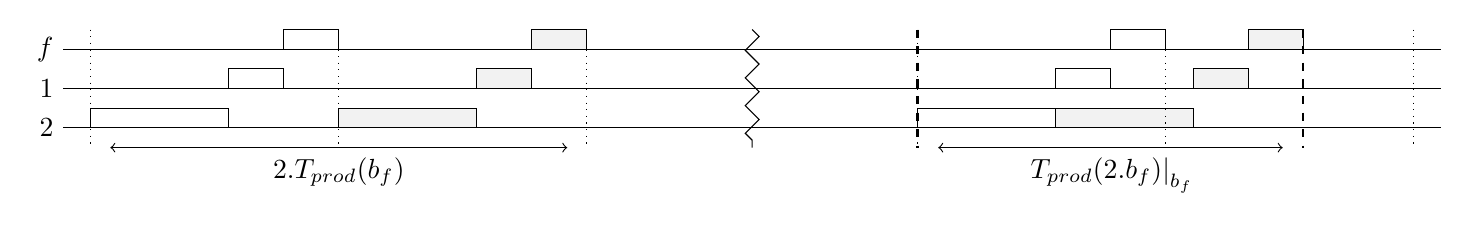
\begin{tikzpicture}[xscale=.7, yscale=.5]
        \draw (0,0) node[left] {$f$} -- (25, 0);
        \draw (0,-1) node[left] {$1$} -- (25, -1);
        \draw (0,-2) node[left] {$2$} -- (25, -2);
        \draw[decorate, decoration=zigzag] (12.5, .5) -- (12.5, -2.5);

        % left
        \draw (.5, -2) rectangle (3, -1.5);
        \draw (3, -1) rectangle (4, -.5);
        \draw (4, 0) rectangle (5, .5);

        \draw[fill=gray!10] (5, -2) rectangle (7.5, -1.5);
        \draw[fill=gray!10] (7.5, -1) rectangle (8.5, -.5);
        \draw[fill=gray!10] (8.5, 0) rectangle (9.5, .5);

        \draw[dotted] (.5, .5) -- (.5, -2.5) node[right] (l1) {};
        \draw[dotted] (5, .5) -- (5, -2.5);
        \draw[dotted] (9.5, .5) -- (9.5, -2.5) node[left] (l2) {};

        \draw[<->] (l1) -- node[below] {$2.T_{prod}(b_f)$} (l2);

        % right
        \draw (15.5, -2) rectangle (18, -1.5);
        \draw (18, -1) rectangle (19, -.5);
        \draw (19, 0) rectangle (20, .5);

        \draw[fill=gray!10] (18, -2) rectangle (20.5, -1.5);
        \draw[fill=gray!10] (20.5, -1) rectangle (21.5, -.5);
        \draw[fill=gray!10] (21.5, 0) rectangle (22.5, .5);

        \draw[dotted] (15.5, .5) -- (15.5, -2.5);
        \draw[dashed, thick] (15.5, .5) -- (15.5, -2.5) node[right] (r1) {};
        \draw[dashed, thick] (22.5, .5) -- (22.5, -2.5) node[left] (r2) {} ;
        \draw[dotted] (20, .5) -- (20, -2.5);
        \draw[dotted] (24.5, .5) -- (24.5, -2.5);

        \draw[<->] (r1) -- node[below] {$\left. T_{prod}(2.b_f)\right|_{b_f}$} (r2);

    \end{tikzpicture}
    \caption{\label{produced_i:2bf}}
\end{figure}

\subsubsection{A first example}

However, the above formula holds for a given bottleneck machine. But we do know that the bottleneck machine depends on the batch size which has been chosen \textit{a priori} : given a batch size $b_f$, we can comptue the production time $T_{prod}(K.b_f)|_{b_f}$. But how can we choose $b_f$ with constraints on the production rate, on the overall production time, and, as well, on the number of items to be produced ? This is not an easy question actually, so let's take an example in order to better understand where the difficulty lies. 

\begin{wrapfigure}[12]{r}{5cm}
    \centering
    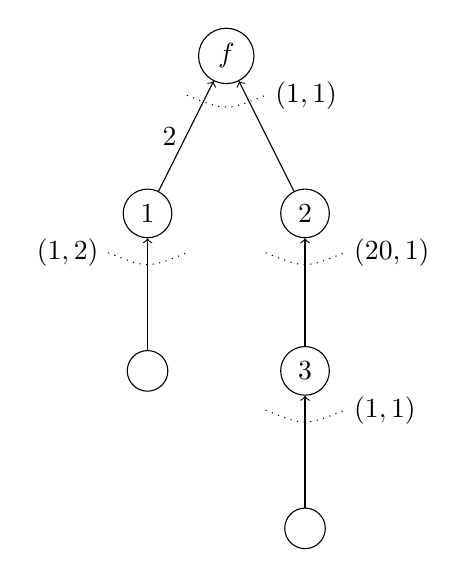
\begin{tikzpicture}
        \draw (0,0) node[draw, circle] (f) {$f$};
        \draw (-1, -2) node[draw, circle] (1) {$1$};
        \draw (-1, -4) node[draw, circle] (RM1) {$\vphantom{1}$};

        \draw (1, -2) node[draw, circle] (2) {$2$};
        \draw (1, -4) node[draw, circle] (3) {$3$};
        \draw (1, -6) node[draw, circle] (RM2) {$\vphantom{1}$};

        \draw[->] (RM1) -- (1);
        \draw[->] (1) -- node[left] {$2$} (f);

        \draw[->] (RM2) -- (3);
        \draw[->] (3) -- (2);
        \draw[->] (2) -- (f);

        \draw[dotted] (-.5, -.5) .. controls (0, -.7) .. (.5, -.5) node[right] {$(1, 1)$};
        \draw[dotted] (-1.5, -2.5) node[left] {$(1, 2)$} .. controls (-1, -2.7) .. (-.5, -2.5);
        
        \draw[dotted] (.5, -2.5) .. controls (1, -2.7) .. (1.5, -2.5) node[right] {$(20, 1)$};
        \draw[dotted] (.5, -4.5) .. controls (1, -4.7) .. (1.5, -4.5) node[right] {$(1, 1)$};
    \end{tikzpicture}
    \caption{\label{produced_i:example1}Example BoM}
\end{wrapfigure}

Let's consider the Bill of Material depicted in figure (\ref{produced_i:example1}) with the following constraints : \begin{enumerate}
    \item Minimum production rate of $X_f^* = \frac{1}{5}$
    \item Maximum production time for a batch $\bar T = 80$
    \item Number of items to be produced $N = 200$
\end{enumerate} We are very used to the first two constraints. The first one gives us a lower bound for the batch size in order for the production rate to be feasible. The second one gives us an upper bound so that the production time of a batch is not greater than the time limit. Computing these bounds is rather easy and we will not discuss them : 
\[
    \begin{split}
        b_f^* &= \max_i\left( \frac{X_f^*T_{si}}{1-X_f^*T_{oi}n_{if}} \right)\\
              &= \max\left(
                    \frac{ \frac{1}{5} . 1 }{1 - \frac{1}{5} . 1 } ;
                    \frac{ \frac{1}{5} . 1 }{1 - \frac{1}{5} . 2 . 2 } ;
                    \frac{ \frac{1}{5} . 20 }{1 - \frac{1}{5} . 1 . 1 } ;
                    \frac{ \frac{1}{5} . 1 }{1 - \frac{1}{5} . 1 . 1 }
                  \right)\\
              &= 5\\
        \bar b_f &= \min_{\mathcal P_k}\left( \frac{\bar T - \sum_{i\in\mathcal P_k}T_{si}}{\sum_{i\in\mathcal P_k}T_{oi}n_{if}}\right)\\
                 &= \min\left(
                        \frac{80 - ( 1 + 1 )}{ 2.2 + 1.1 } ;
                        \frac{80 - ( 1 + 20 + 1 )}{ 1.1 + 1.1 + 1.1 } ;
                    \right)\\
                 &= 15.6
    \end{split}
\]

Which tells us that we need to choose our batch size so that $b_f\in [ 5, 15 ]$. Since we want to produce $N=200$ items, we should repeat a certain number of times the production of such bacthes untill we reach $200$ items. On possible way would be to produce $40$ times a batch of $5$ items (since $40\times 5 = 200$), or produce $25$ times batches of $8$ (since again $25\times 8=200$). In fact, the only multiples of $200$ witin the interval $[5, 15]$ are $\{ 5, 8, 10 \}$. Let's study each one of these cases !

For each cases, we can write the equation (\ref{produced_i:tprod}) as \[
    \begin{split}
        T_{prod}(200)|_{bf=5} &= T_{prod}(5) + 39.T_b(5)\\
        T_{prod}(200)|_{bf=8} &= T_{prod}(8) + 39.T_b(10)\\
        T_{prod}(200)|_{bf=10} &= T_{prod}(8) + 39.T_b(10)\\
    \end{split}
\] where $T_{prod}(b_f)$ can be computed as \[
    T_{prod}(b_f) = \max_{\mathcal P_k}\left( \sum_{i\in\mathcal P_k} ( T_{si} + T_{oi}n_{if} ) \right) = \max ( 2 + 5.b_f ; 22 + 3.b_f )
\] and \[ T_b(b_f) = \max( 1 + 1.b_f ; 1 + 2.2.b_f ; 20 + 1.b_f ; 1 + 1.b_f ) = \max( 1 + 4b_f ; 20 + b_f ) \]

Using these formulas, we easily get the following results : \begin{center}
    \begin{tabular}{|c|c|c|c|}
        \hline
        $b_f$ & $T_{prod}(b_f)$ & $T_b(b_f)$ & $T_{prod}(200)|_{b_f}$\\\hline
        $5$ & $37$ & $25$ & $1012$ \\\hline
        $8$ & $46$ & $33$ & $838$ \\\hline
        $10$ & $52$ & $41$ & $831$ \\\hline
    \end{tabular}
\end{center} Which means that, for this way of producing $200$ items, using a batch size of $10$ items is the quicker (it turns out to be the biggest batch size but this is just a particular case). However, there are other ways of getting to $200$ ! For example, we may want to produce $13$ batches of $15$ and a batch of $5$, since $200 = 13\times 15 + 5$. Looking at figure (\ref{produced_i:gant}), we realise that we can compute the time needed to produce $200$ items in that way by first computing the time to produce $13$ bacthes of $15$ and then add the difference between the needed time to produce a batch of $5$ and the time at which the bottleneck machine can start.

We get that : \[
    \begin{split}
        T_{prod}(15) &= 77\\
        T_b(15) &= 61\\
        T_{prod}(195)|_{bf=15} &= 77 + 12.61 = 809\\
        T_{prod}(5) &= 37\\
        T_b(5) &= 25
    \end{split}
\] And, it holds that the delay represented by the red arrow in figure (\ref{produced_i:gant}) can be computed as the production time of the bottleneck machine $T_b(5)$ minus the production time of machine $f$, which yields $25 - 16 = 9$. We can now compute the final, overall, production time which is : $809 + 9 + 6 = 824$ ! Which is less than what we had previously found. 

\begin{figure}[h!]
    \centering
    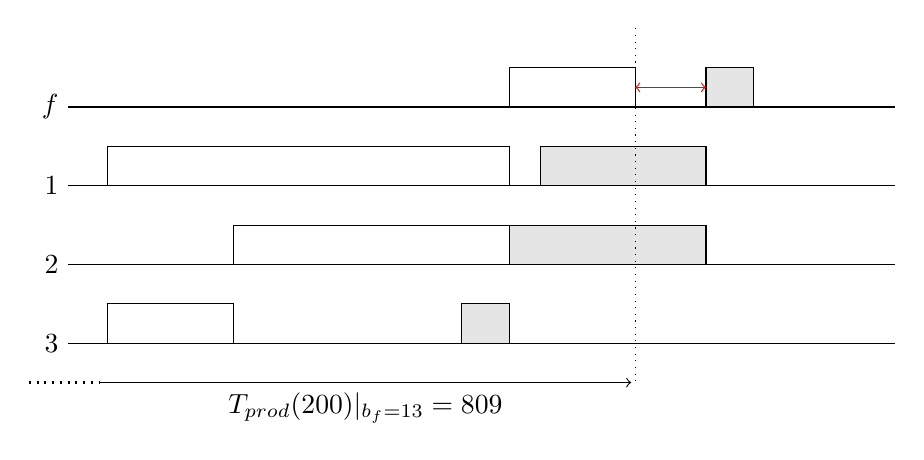
\begin{tikzpicture}[xscale=.1]
        \foreach \y/\m in {0/$f$, -1/$1$, -2/$2$, -3/$3$} \draw (-5,\y) node[left] {\m} -- (100, \y);

        \draw (0,-3) rectangle (16, -2.5);
        \draw (16,-2) rectangle (16 + 35, -1.5);
        \draw (0,-1) rectangle (51, -.5);
        \draw (51, 0) rectangle (51 + 16, .5);

        \draw[fill=gray!20] (51, -2) rectangle (51 + 25, -1.5);
        \draw[fill=gray!20] (51 + 25 - 21, -1) rectangle (51 + 25, -.5);
        \draw[fill=gray!20] (51 - 6, -3) rectangle (51, -2.5);
        \draw[fill=gray!20] (51 + 25, 0) rectangle (51 + 25 + 6, .5);

        \draw[dotted] (67, 1) -- (67, -3.5);

        \draw[->] (-1, -3.5) -- node[below] {$T_{prod}(200)|_{b_f = 13} = 809$} (66.5, -3.5);
        \draw[dotted, thick] (-10, -3.5) -- (-1, -3.5);
        
        \draw[<->, red] (67, .25) -- (67 + 9, .25);
    \end{tikzpicture}
    \caption{\label{produced_i:gant}GANT diagram corresponding to the production of $200 = 13\times 15 + 5$ items}
\end{figure}

Finding the optimal batch size is not easy to be done by hand and we usually use approximation techniques to find a solution. 

\subsubsection{Approximate solution}

Let us define our coefficient $K$ as $\frac{N}{b_f}$ and let's assume that this number is an integer number. Then, assuming that we know \textit{a priori} the bottleneck machine $b$, it holds that \[ \begin{split}
    T_{prod}(N)|_{b_f} &= \sum_{i\in\mathcal P_k} ( T_{si} + T_{oi}n_{if}b_f ) + \left( \frac{N}{b_f} - 1 \right)(T_{sb} + b_fT_{ob}n_{bf})\\
    &= \sum_{i\in\mathcal P_k} T_{si} + b_f\left( \sum_{i\in\mathcal P_k} T_{oi}n_{if} - T_{ob}n_{bf} \right) + NT_{ob}n_{bf} + \frac{N}{b_f}T_{sb}
    \end{split}
\] which is just a re-writing of the previously introduced equations. This function of $b_f$ is convex, we can find its global minimum by first relaxing the "integer" constraint and derivating this function and solving $\nabla . = 0$. We get
\[
    \frac{\partial .}{\partial b_f} = \sum_{i\in\mathcal P_k} T_{oi}n_{if} - T_{ob}n_{bf} - \frac{N}{b_f^2}T_{sb}
\] and \[
    \nabla . = 0 \Leftrightarrow b_f^\circ = \sqrt{ \frac{T_{sb}}{\sum_{i\in\mathcal P_k} T_{oi}n_{if} - T_{ob}n_{bf} } }
\]
This results gives us the optimal batch size we should use \textbf{given the bottleneck machine considered}. However, we know that the bottleneck changes with the batch size. In fact, imagine a situation in which the bottleneck machine changes for a given batch size, say $\tilde b_f$. And imagine a situation in which, for $b_f > \tilde b_f$, we have a convex function like the red one in figure (\ref{produced_i:convex}), and that, on the other hand, for $b_f < \tilde b_f$, we have a convex function like the black one in the same figure. Using that formula will yield one of the two extremum depending on which machine we assume to be the bottleneck machine...

\begin{figure}[h!]
    \centering
    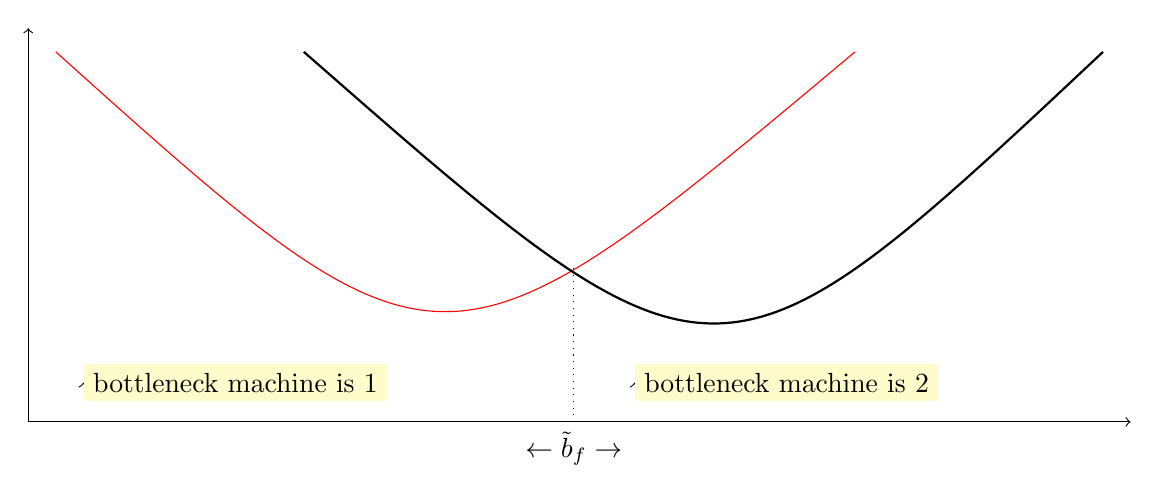
\begin{tikzpicture}[xscale=.7]
        \draw[<->] (0, 5) |- (20, 0);

        \draw[->] (1, .5) node[fill=yellow!20, right] {bottleneck machine is $1$};
        \draw[->] (11, .5) node[fill=yellow!20, right] {bottleneck machine is $2$};

        \draw[red] (0.5, 4.7) .. controls (7.5, .3) .. (15, 4.7);
        \draw[thick] (5, 4.7) .. controls (12.5, .1) .. (19.5, 4.7);
        \draw[dotted] (9.9, 0) node[below] {$\leftarrow\tilde b_f\rightarrow$} -- ++(0, 1.95);
    \end{tikzpicture}
    \caption{\label{produced_i:convex}Two different convex functions for finding "optimal" batch size}
\end{figure}

\subsubsection{Upper bound}

As previously said, computing the exact production time needed to produce $N$ items isn't an easy thing to do. However, a good upper bound for the production time, given a batch size $b_f$, can be computed as \[ T_{prod}(N)|_{b_f}\le T_{prod}(b_f) + \left( \left\lceil \frac{N}{b_f} \right\rceil - 1 \right)T_b(b_f) \] The error we're making in our estimate is then proportionnal to $\left\lceil \frac{N}{b_f} \right\rceil b_f - N$ where $\left\lceil \frac{N}{b_f} \right\rceil b_f$ represents the number of items for which we computed the production time and $N$ the aimed number of items. 

\subsection{Pull systems}

Concerning production systems which use the Kanban approach (also refered as pull systems), we can find a somehow analogous formula to compute an upper bound for the production time of $N$ items.

From the previous sections, we know that the ratio $D/D_i$ gives us the number of batches that machine $i$ delivers during a time window $D$. Thus, the working time of machine $i$ can be computed as \[ T_{wi} = \frac{D}{D_i}(T_{si}+T_{oi}b_i) \] Which equals, if we consider the batch sizing as $b_i = b_f n_{if}$, \[ \frac{D}{\frac{b_f}{X_f^{max}(b_f)}} (T_{si} + T_{oi}n_{if}) = D\frac{X_f^{max}(b_f)}{\frac{b_f}{T_{si}+T_{oi}n_{if}b_f}} \] since $D_i = D, \forall i$ and $D = b_f / X^{max}_f(b_f)$. Finally, noting that $X_f^{max} = \min\left( \frac{b_f}{T_{si} + T_{oi}b_fn_{if}} \right)$, we conclude that in any case : \[ T_{wi} \le D \] Thus, it stands that, since the time to produce the first batch is given by $L.D$ where $L$ is the level of the Bill of Material, an upper bound for the production time of $N$ items using batch sized as $b_i = b_fn_{if}$ in the pull production system is :
\[
    T_{prod}^{pull}(N)|_{b_f} = LD + \left\lceil \frac{N}{b_f} - 1 \right\rceil D
\]
This is very analogous to the previous formula obtained when dealing with push systems since here, the production cycle $D$ is determined by the bottleneck machine ($D = T_b(b_f)$). 

\subsection{Conclusion}

We end up with two estimates for an upper bound of the time to produce $N$ items which are : 
\[
    \begin{split}
        T_{prod}^{push}(N)|_{b_f} &\le T_{prod}(b_f) + \left( \left\lceil \frac{N}{b_f} \right\rceil - 1 \right)T_b(b_f)\\
        T_{prod}^{pull}(N)|_{b_f} &\le LD + \left( \left\lceil \frac{N}{b_f}\right\rceil - 1 \right) T_b(b_f)
    \end{split}
\]

And it can be easily seen that $T_{prod}^{push}(b_f) \le LD$ which imples the following relation between our two upper bounds : 
\[ T_{prod}^{push}(N)|_{b_f} \le T_{prod}^{pull}(N)|_{b_f} \]
But since our goal is to find a "reasonable" time to be considered for the production of $N$ items, for instance to tell our consumer that the production will be ready by that time and that he should come pick up our final products, one may always use the second formula even for \textit{push} systems since (1) it is an upper bound of the production time and (2) we end with a uniform formula. 

\subsection{Computing upper bounds : one final example}

\begin{wrapfigure}[14]{l}{4cm}
    \centering
    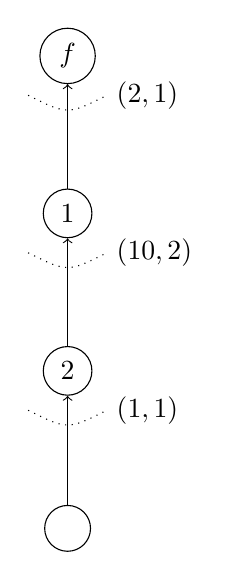
\begin{tikzpicture}
        \draw (0, 0) node[draw, circle] (f) {$f$};
        \draw (0, -2) node[draw, circle] (1) {$1$};
        \draw (0, -4) node[draw, circle] (2) {$2$};
        \draw (0, -6) node[draw, circle] (RM) {$\vphantom{j}$};

        \draw[dotted] (-.5, -.5) .. controls (0, -.75) .. (.5, -.5) node[right] {$(2, 1)$};
        \draw[dotted] (-.5, -2.5) .. controls (0, -2.75) .. (.5, -2.5) node[right] {$(10, 2)$};
        \draw[dotted] (-.5, -4.5) .. controls (0, -4.75) .. (.5, -4.5) node[right] {$(1, 1)$};

        \draw[<-] (f) -- (1);
        \draw[->] (2) -- (1);
        \draw[<-] (2) -- (RM);
    \end{tikzpicture}
    \caption{\label{produced_i:simple_bom}Example}
\end{wrapfigure}

Consider figure (\ref{produced_i:simple_bom}) which represents a very simple bill of material. Let's assume that one client orders $N = 70$ final products. When should we tell him to come back to pick up his goods ? We will do the computations studying various batch sizes among $10, 7$ and $6$. 

\subsubsection{Using push systems}

Using the previously established formula, we can compute an upper bound of the time needed to produce $N=70$ items like so :
\[
    T_{prod}^{push}(70)|_{b_f = 10} = (\underline{1 + 1.10} + \underline{ 10 + 2.10 } + \underline{ 2 + 1.10 } ) + (7-1)(10 + 2.10) = 233
\] since with $b_f = 10$, machine number $1$ is the bottleneck machine. Note that, in this situation, the computed upper bound is actually the "supremum" (the best upper bound we can found) which coincides with the exact value of $T_{prod}^{push}$ since $70$ is a multiple of $10$. 

Similar computations gives the following results : 
\[
    \begin{split}
        T_{prod}^{push}(70)|_{b_f = 7} &= 257\\
        T_{prod}^{push}(70)|_{b_f = 6} &\le 279\\
    \end{split}
\]
And note that, in the latter case, the result is an upper bound which differs from the exact value of the production time needed since $6$ is not a divisor of $70$. Actually, we are estimating our upper bound by computing the time needed to produce $6\times 12 = 72$ items instead of $70$ since $\lceil 70 / 6 \rceil = 12$. 

\subsubsection{Using pull systems}

Using the corresponding formula for the pull systems, we can compute upper bounds in the same way. (Note that the formula can be rewritten as $T_{prod}^{pull}(N)_{b_f} = \left( L-1+\left\lceil \frac{N}{b_f} \right\rceil \right) T_b(b_f)$ which is handier to compute by hand...). Doing so, we get the following results : 

\[
    \begin{split}
        T_{prod}^{pull}(70)|_{b_f = 10} &\le (3 - 1 + 7).30 = 270\\
        T_{prod}^{pull}(70)|_{b_f = 7} &\le 288\\
        T_{prod}^{pull}(70)|_{b_f = 6} &\le 308\\
    \end{split}
\]

Which gives as expected greater upper bounds but sufficiently good ones.

\subsubsection{Optimal batch sizing ?}

Just like we did in the section dedicated to push systems, and since we know that we can use one uniformed formula, let's suppose $N/b_f$ to be integer and let's assume knowing the bottleneck machine corresponding to the optimal batch size, our upper bound can be given by \[
    \begin{split}
        T_{prod}(N)_{b_f} &= \left(L - 1 \frac{N}{b_f}\right)T_b(b_f) \\
        &= \left(L-1\frac{N}{b_f}\right) ( T_{sb} + T_{ob}b_fn_{bf} ) \\
        &= \frac{N}{b_f}T_{sb} + (L-1)T_{ob}b_fn_{b_f} + (L-1)T_{sb} + NT_{ob}n_{bf}
    \end{split}
\]
And let's take the derivative of this function with respect to $b_f$, it yields 
\[
    \frac{dT_{prod}}{db_f} = -\frac{N}{b_f^2} + (L-1)T_{ob}b_fn_{bf}
\]
Which is convex and yields the optimal solution \[ b_f^\circ = \sqrt{ \frac{NT_{sb}}{ (L-1)T_{ob}n_{bf} } } \]
But keep in mind that, similarly to what have been said in the previous section, this formula holds only if the bottleneck machine was well the one we had supposed it would be. That is, we have to check \textit{a posteriori} that the bottleneck machine we considered for our computation is well the one corresponding to the batch size $b_f^\circ$. 

Looking back at our example, we obtain the "optimal" batch size (supposing that $1$ will be the bottleneck machine) as $b_f^\circ = \sqrt{ \frac{70.10}{2.2} } \approx 14$. Using such a batch size\footnote{which is relevant since the bottleneck machine associated to that batch size is well machine $1$} will result in the "smallest" production time estimate using the established formula which are \[
    \begin{split}
    T_{prod}^{push}(70)|_{b_f = 14} &= 221\\
    T_{prod}^{push}(70)|_{b_f = 14} &= 266\\
    \end{split}
    \]

\section{Arbitrary batch sizing}

Our final consideration concerning the computation of the time needed to produce a fixed number of items $N$ is the one related to the situation in which $b_i\ne b_fn_{if}$. We have seen that the only way of producing using an arbitrary batch size is to use the Kanban system. In this case, we are dealing with different batch sizes for each machine $b_i$ which are arbitrary choosen. We have already established that $\frac{D}{D_i}=K_i$ gives us the number of batches of product $i$ produced during the time window $D$. Thus, $K_ib_i$ returns the number of items $i$ produced during one production cycle $D$ and $\left\lceil \frac{N}{K_fb_f} \right\rceil$ equals the number of production cycle $D$ needed in order to produce $N$ items. Thus, the following formula holds:  
\[
    T_{prod}(N)|_{\underline b} = LD + \left(\left\lceil \frac{N}{K_fb_f} \right\rceil - 1\right)D
\]
Which is a generalization of the previous formula when $b_i = b_fn_{if}$ since in this case we have $K_f = 1$. 